%%=============================================================================
%% Inleiding
%%=============================================================================

\chapter{\IfLanguageName{dutch}{Inleiding}{Introduction}}
\label{ch:inleiding}

IT-bedrijven willen hun klanten sneller te hulp kunnen schieten, betere software leveren. Maar ze worstelen nog vaak met deadlines die verstrijken en veel problemen tijdens de oplevering van software. Gelukkig is er doorheen de jaren al veel progressie gemaakt door principes zoals Agile en DevOps toe te passen. Agile leidt tot een betere samenwerking tussen business en de IT. DevOps gaat dan weer een stapje verder en is een mindset om de samenwerking tussen alle afdelingen binnen een IT-bedrijf vlotter te maken. 
Een Continuous Integration en Continuous Delivery (CI/CD) pipeline opzetten is een vast onderdeel van DevOps en zou de werking van een bedrijf ten goede komen. Een CI/CD pipeline zorgt voor de automatisatie van testen, builds en deployment en heeft als grote voordeel dat er sneller wijzigingen doorgevoerd kunnen worden, alsook de tijd dat een applicatie niet runt -'downtime' in IT genoemd- kleiner wordt.

Uit onderzoek - uitgevoerd door DZone , een gerenommeerd vakblad binnen IT - blijkt dat DevOps steeds meer ingeburgerd raakt in de bedrijfscultuur. 48\% van de ondervraagden in 2019 werkt het Operations team van het bedrijf aan aan een Continuous Delivery pipeline, een stijging van 7\% in vergelijking met 2018.
De stijging is te wijten aan het management dat geloofd in de mindset van DevOps. Van de 527 technologie specialisten heeft bij 54\% van hen de steun van het management. Maar er is natuurlijk nog een hele weg af te leggen.
Als we verder naar het onderzoek kijken blijkt dat er een duidelijk verschil is tussen de implementatie van DevOps en de implementatie van een CI/CD pipeline. 
Voor Continuous Integration 31\% past voor elk project een Continuous Integration pipeline toe en 33\% heeft een CI pipeline voor enkele projecten.
Slechts 14\% van de ondervraagden bevestigt dat ze voor elk project aan Continuous Delivery doen. Er is zelfs een daling ten opzichte van 2018.
28 procent heeft voor enkele projecten zo een Continuous Delivery pipeline. 
Hieruit kan men besluiten dat CI meer ingeburgerd is dan CD. In 58\% van de gevallen volgen de Continuous Integration processen niet door naar Continuous Delivery. De belangrijkste redenen voor deze 'gap' zijn de moeilijkheid van de configuration setup, de moeilijkheden van user acceptance testing (de laatste fase binnen de software testing waarbij echte gebruikers de software testen) en de automated testing.
Volgens 47\% van de 527 technologie specialisten was dit te wijten aan de bedrijfscultuur die niet klaar is om Continuous Delivery toe te passen, in 2018 was dit nog 45\%.
%TODO: Referentie nog toevoegen voor Jordan Baker!
%TODO: Referentie met DevOps magazine nog toevoegen! Uitzoeken welk soort referentie het is! Want met die auteurs weet ik het niet goed!
Zoals u kan zien op Figuur\ref{img-survey-cicd} is er nog heel wat werk aan de winkel, maar er is toch al wat verbetering vastgesteld ten opzichte van vorige jaren. Dit bewijst ook dat een CI/CD pipeline en DevOps in het algemeen niet zo makkelijk op te zetten is. Technologisch is het vandaag mogelijk om een pipeline op te stellen, maar de mindset binnen het bedrijf moet meewerken om dit tot een goed eind te brengen.
Deze scriptie gaat echter niet al te diep in hoe de DevOps cultuur binnen een bedrijf toe te passen, maar zal vooral het technische luik onder de loep nemen. Het bedrijf Amista zou graag een gepersonaliseerde vergelijking en handleiding hebben hoe men technisch een CI/CD pipeline opstart.

%TODO: de autocite nog compleet maken!
\begin{figure}	
    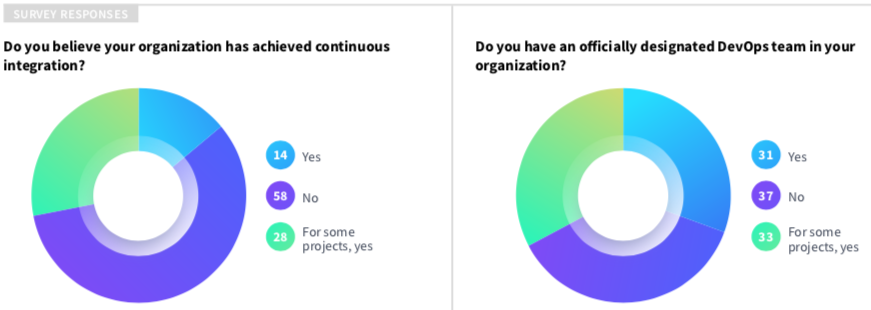
\includegraphics[scale=0.65]{survey-DZone-cicd}
    \caption{Deel van DZone's survey ~\autocite{}} \label{img-survey-cicd}
\end{figure}

Amista is een groeiend bedrijf binnen IT consultancy. Het is een dochterbedrijf van Boutique dat zich toespitst op SAP. Sinds hun vijfjarig bestaan werken er al 60 personen voor Amista. Ze hebben Infrabel, Alcopa, Danone, AG Real Estate en nog anderen tot hun cliënteel, zoals op hun site te lezen valt ~\autocite{Amista2018}.
Ze zijn in twee landen actief, Frankrijk en België, maar werken ook samen met mensen uit India.
Amista heeft zich verdiept in de Sales, Marketing en Service Management takken van bedrijven. Ze helpen hun klanten ook op gebied van Innovation, Integration, HCM Services (implementatie van succesfactoren binnen de HR afdeling) en Digital Learning.
De missie van Amista is om samen met hun klanten innovatieve en kwalitatieve oplossingen aan te bieden met behulp van het volledige gamma dat SAP te bieden heeft.
Omdat Amista graag de wensen van hun klanten zo goed mogelijk probeert te vervullen, proberen ze zelf zo innovatief mogelijk te zijn. Ze spelen met het idee om een CI/CD pipeline op te zetten voor de software development.

Om een Continuous Integration en Continuous Delivery pipeline op te stellen zijn er vandaag veel tools beschikbaar.
Deze thesis zal verschillende build schedulers vergelijken op basis van snelheid, geheugen-verbruik, hoeveelheid beschikbare documentatie en configureerbaarheid met de huidige set-up die Amista gebruikt.
Aan de hand van de 'winnende' build scheduler wordt er een handleiding beschreven om een pipeline op te zetten binnen een SAPUI5 webapplicatie dat verbonden is met SAP HANA en gehost wordt op SAP Cloud Platform.

%De inleiding moet de lezer net genoeg informatie verschaffen om het onderwerp te begrijpen en in te zien waarom de onderzoeksvraag de moeite waard is om te onderzoeken. In de inleiding ga je literatuurverwijzingen beperken, zodat de tekst vlot leesbaar blijft. Je kan de inleiding verder onderverdelen in secties als dit de tekst verduidelijkt. Zaken die aan bod kunnen komen in de inleiding~\autocite{Pollefliet2011}:
%
%\begin{itemize}
%  \item context, achtergrond
%  \item afbakenen van het onderwerp
%  \item verantwoording van het onderwerp, methodologie
%  \item probleemstelling
%  \item onderzoeksdoelstelling
%  \item onderzoeksvraag
%  \item \ldots
%\end{itemize}

\section{\IfLanguageName{dutch}{Probleemstelling}{Problem Statement}}
\label{sec:probleemstelling}

Amista heeft enkele klanten waar ze SAPUI5 webapplicaties voor maken, dit wordt vaak gecombineerd met een SAP HANA database dat gebruik maakt van Node.js en wordt allemaal gehost op SAP Cloud Platform.
Elk bedrijf wil het beste voor zijn klanten. Voor een software consultancy bedrijf, zoals Amista, staat de service en het project dat de klant voor ogen heeft centraal en doen ze er alles aan om in te spelen op de noden en wensen van hun klanten.
Voor projecten wordt er momenteel een datum afgesproken voor oplevering, hier komt vaak veel stress en problemen bij kijken. Om dit te vermijden kan een Continuous Integration en Continuous Delivery pipeline helpen. Ook is het niet makkelijk om met de huidige gang van zaken wijzigingen van de klanten door te voeren. Dankzij een CI/CD pipeline kan men sneller wijzigingen doorvoeren en krijgt men sneller feedback van de klant.
Een levensecht voorbeeld kan dit iets duidelijker maken.

\newline{}Amista heeft een klant, Appel genaamd. Deze klant had in het verleden wat moeilijkheden met opleveringen van projecten en wijzigen van projecten. Daarom hadden ze besloten om een policy toe te passen waarbij de opleveringsdata gebundeld werden en elke twee weken te releasen. Het was dus niet mogelijk om een wijziging door te voeren als de opleveringsdag verstreken was, dan moet men twee weken wachten. 
Appel is een internationale speler en heeft vestigingen over heel de wereld. In één van de landen is het verplicht dat grote bedrijven de belastingen online invullen. Als ze dit niet doen krijgen ze grote boetes. De overheid voorziet hiervoor een speciaal certificaat. De tool voor de belastingaangifte stond op SAP Cloud Platform waar Amista verantwoordelijk voor is. Het certificaat wordt vernieuwd op SAP Cloud Platform op de opleveringsdatum, maar de build loopt mis. Er falen verschillende processen en de applicatie loopt vast. Ze zoeken het probleem uit en vinden dat er een parameter in de backend moet vernieuwd worden. Hier was Amista echter niet verantwoordelijk voor en wist bijgevolg ook niet van het bestaan van deze parameter. Omdat de policy van Appel voorschrijft dat er om de twee weken ee release van de wijzigingen mag doorgevoerd worden is het bedrijf niet voorbereid op onverwachte dingen. Uiteindelijk hebben ze met veel moeite iemand kunnen bereiken die de parameter in de backend vernieuwd heeft en kon zorgen voor een nieuwe release. Ondertussen  had Appel schrik voor de grote boete die boven het hoofd hing.
Met een Continuous Integration en Continuous Delivery pipeline zou dit euvel in no-time opgelost kunnen raken. Met voldoende en goede testen zal de pipeline ook aangeven dat er een probleem is en zal de wijziging nooit productie halen. Het probleem had dus vermeden kunnen worden met 0 downtime.
(Bovenstaand voorbeeld bevat fictieve namen).

\newline{}Om een CI/CD pipeline op te zetten binnen de hierboven beschreven omgeving is er nog niet veel informatie terug te vinden. Het probleem ligt hem in de combinatie van specifieke tools die gebruikt worden. Om te weten welke build scheduler het beste bij deze omgeving zou passen moeten er specifieke zaken onderzocht worden. Op internet is niet veel informatie terug te vinden welke build scheduler het beste zou passen binnen deze omgeving, ook niet om een CI/CD pipeline op te zetten. Daarom wil Amista heel graag een gepersonaliseerde vergelijking en handleiding om een Continuous Integration en Continuous Delivery pipeline op te zetten zodat ze hun klanten beter kunnen helpen.

%Uit je probleemstelling moet duidelijk zijn dat je onderzoek een meerwaarde heeft voor een concrete doelgroep. De doelgroep moet goed gedefinieerd en afgelijnd zijn. Doelgroepen als ``bedrijven,'' ``KMO's,'' systeembeheerders, enz.~zijn nog te vaag. Als je een lijstje kan maken van de personen/organisaties die een meerwaarde zullen vinden in deze bachelorproef (dit is eigenlijk je steekproefkader), dan is dat een indicatie dat de doelgroep goed gedefinieerd is. Dit kan een enkel bedrijf zijn of zelfs één persoon (je co-promotor/opdrachtgever).

\section{\IfLanguageName{dutch}{Onderzoeksvraag}{Research question}}
\label{sec:onderzoeksvraag}

\begin{itemize}
    \item Wat zijn de voor- en nadelen van een CI/CD pipeline in het algemeen en specifiek voor Amista?
    \item Is het mogelijk om een Continuous Integration en Continuous Delivery pipeline te implementeren voor de ontwikkelingen van een SAPUI5 applicatie op SAP Cloud Platform?
    \item Welke tools moeten we gebruiken om een CI/CD pipeline op SAP Cloud Platform te implementeren als we vergelijken op snelheid, geheugen-verbruik, configureerbaarheid en hoeveelheid documentatie.
    \item Hoe kunnen we deze implementatie tot een succes brengen?
    
\end{itemize}
%Wees zo concreet mogelijk bij het formuleren van je onderzoeksvraag. Een onderzoeksvraag is trouwens iets waar nog niemand op dit moment een antwoord heeft (voor zover je kan nagaan). Het opzoeken van bestaande informatie (bv. ``welke tools bestaan er voor deze toepassing?'') is dus geen onderzoeksvraag. Je kan de onderzoeksvraag verder specifiëren in deelvragen. Bv.~als je onderzoek gaat over performantiemetingen, dan 

\section{\IfLanguageName{dutch}{Onderzoeksdoelstelling}{Research objective}}
\label{sec:onderzoeksdoelstelling}

Deze thesis zou als hoofddoel een proof-of-concept zijn hoe een CI/CD pipeline te gebruiken in de dagelijkse werking van Amista. 
Maar deze thesis gaat ook op zoek naar de beste tools om de pipeline op te bouwen rekening houdend met snelheid, geheugen-verbruik, configureerbaarheid met de tools die Amista gebruikt en hoeveelheid documentatie er te vinden is.
%Wat is het beoogde resultaat van je bachelorproef? Wat zijn de criteria voor succes? Beschrijf die zo concreet mogelijk. Gaat het bv. om een proof-of-concept, een prototype, een verslag met aanbevelingen, een vergelijkende studie, enz.

\section{\IfLanguageName{dutch}{Opzet van deze bachelorproef}{Structure of this bachelor thesis}}
\label{sec:opzet-bachelorproef}

% Het is gebruikelijk aan het einde van de inleiding een overzicht te
% geven van de opbouw van de rest van de tekst. Deze sectie bevat al een aanzet
% die je kan aanvullen/aanpassen in functie van je eigen tekst.

De rest van deze bachelorproef is als volgt opgebouwd:

In Hoofdstuk~\ref{ch:stand-van-zaken} wordt een overzicht gegeven van de stand van zaken binnen het onderzoeksdomein, op basis van een literatuurstudie.

In Hoofdstuk~\ref{ch:methodologie} wordt de methodologie toegelicht en worden de gebruikte onderzoekstechnieken besproken om een antwoord te kunnen formuleren op de onderzoeksvragen.

De set-up van de omgeving wordt in detail besproken in Hoofdstuk~\ref{ch:voorbeeldapplicatie}.

Een vergelijking tussen de verschillende build schedulers kan men vinden in Hoofdstuk~\ref{ch:vergelijking-tools}

In Hoofdstuk~\ref{ch:handleiding} wordt er een gepersonaliseerde handleiding gegeven om met de beste build scheduler een CI/CD pipeline te implementeren.

De waarom-vraag is minstens even belangrijk als de hoe-vraag. Concreet: wat zijn de voor- en nadelen van een CI/CD pipeline te integreren in het algemeen en specifiek voor Amista? Een antwoord op deze vragen kan je in Hoofdstuk~\ref{ch:voor-en-nadelen-cicd}.

In Hoofdstuk~\ref{ch:conclusie}, tenslotte, wordt de conclusie gegeven en een antwoord geformuleerd op de onderzoeksvragen. Daarbij wordt ook een aanzet gegeven voor toekomstig onderzoek binnen dit domein.